% Makros zur Kompatibilitaet mit Onlinemodul: 
 \providecommand{\MoIl}[1][]{\mbox{}#1]\mathopen{}} 
 \providecommand{\MoIr}[1][]{#1[\mbox{}} 
 \providecommand{\MIntvlSep}{;} 
 \providecommand{\MElSetSep}{\, ; \, } 
 \begin{MAufgabe}{Lineare Betrags(un)gleichungen}{vr, 2016, MaTeX}
L\"osen Sie die Gleichung
$$
 \MDS 2\left| 6\, x \right|+2\, x - 1=  \left| 1 - 2\, x \right|  - 3\, x - 3
$$  

\ifLsg\MLoesung

Im ersten Schritt k\"onnen die Terme au\ss{}erhalb der Betragszeichen zusammengefasst werden:

\begin{align*} 
 2\left| 6\, x \right|+2\, x - 1=  \left| 1 - 2\, x \right|  - 3\, x - 3\\ 
\Leftrightarrow5\, x - \left|2\, x - 1\right| + 12\, \left|x\right| + 2= 0 
 \end{align*}

F\"ur diese Gleichung haben wir 4 F\"alle zu unterscheiden: 
\begin{enumerate}
\item $ \MDS 
\begin{cases} 
 0 \leq 6\, x\\ 
0 \leq 1 - 2\, x
 \end{cases}
\Leftrightarrow 0 \leq x \wedge x \leq \frac{1}{2}\Leftrightarrow x \in [ 0 \, \MIntvlSep \, \frac{1}{2}]$ 
\item $ \MDS 
\begin{cases} 
 0 \leq 6\, x\\ 
1 - 2\, x < 0
 \end{cases}
\Leftrightarrow \frac{1}{2} < x\Leftrightarrow x \in \MoIl  \frac{1}{2} \, \MIntvlSep \, \infty\MoIr $ 
\item $ \MDS 
\begin{cases} 
 6\, x < 0\\ 
0 \leq 1 - 2\, x
 \end{cases}
\Leftrightarrow x < 0\Leftrightarrow x \in \MoIl  -\infty \, \MIntvlSep \, 0\MoIr $ 
\item $ \MDS 
\begin{cases} 
 6\, x < 0\\ 
1 - 2\, x < 0
 \end{cases}
 \mbox{ : keine L\"osung. Diese Bedingung ist nirgendwo erf\"ullt.}$ 
\end{enumerate} 
Der 4. Fall ist nirgendwo erf\"ullt. Betrachte weiter nur die restlichen F\"alle.
 
 Fallunterscheidung: 

 \begin{enumerate} 
 \item Sei $ \MDS x\in[ 0 \, \MIntvlSep \, \frac{1}{2}]$. 
 In diesem Fall gilt: 
  $ \MDS \left| 6\, x\right|=6\, x$ und $ \MDS \left| 1 - 2\, x\right|=1 - 2\, x$. \\ 
 Damit ist die Gleichung 
 $$ 
5\, x - \left|2\, x - 1\right| + 12\, \left|x\right| + 2= 0
$$
 \"aquivalent zur Gleichung
 $$ 
2\left(6\, x\right)-\left( 1 - 2\, x\right)+5\, x+2= 0 
$$  
$$ 
 \Leftrightarrow 19\, x + 1= 0 
$$  
$$ \Leftrightarrow x = - \frac{1}{19} . 
 $$ 
 Die L\"osung muss auch die Fallbedingung $x\in [ 0 \, \MIntvlSep \, \frac{1}{2}] $ erf\"ullen. Die gefundene L\"osung $x=- \frac{1}{19}$ erf\"ullt die Fallbedingung  $x\in [ 0 \, \MIntvlSep \, \frac{1}{2}]$ nicht und deshalb ist  $$
 \mathcal{L}_{1}=\emptyset 
 $$ 
\item Sei $ \MDS x\in\MoIl  \frac{1}{2} \, \MIntvlSep \, \infty\MoIr $. 
 In diesem Fall gilt: 
  $ \MDS \left| 6\, x\right|=6\, x$ und $ \MDS \left| 1 - 2\, x\right|=2\, x - 1$. \\ 
 Damit ist die Gleichung 
 $$ 
5\, x - \left|2\, x - 1\right| + 12\, \left|x\right| + 2= 0
$$
 \"aquivalent zur Gleichung
 $$ 
2\left(6\, x\right)-\left( 2\, x - 1\right)+5\, x+2= 0 
$$  
$$ 
 \Leftrightarrow 15\, x + 3= 0 
$$  
$$ \Leftrightarrow x = - \frac{1}{5} . 
 $$ 
 Die L\"osung muss auch die Fallbedingung $x\in \MoIl  \frac{1}{2} \, \MIntvlSep \, \infty\MoIr  $ erf\"ullen. Die gefundene L\"osung $x=- \frac{1}{5}$ erf\"ullt die Fallbedingung  $x\in \MoIl  \frac{1}{2} \, \MIntvlSep \, \infty\MoIr $ nicht und deshalb ist  $$
 \mathcal{L}_{2}=\emptyset 
 $$ 
\item Sei $ \MDS x\in\MoIl  -\infty \, \MIntvlSep \, 0\MoIr $. 
 In diesem Fall gilt: 
  $ \MDS \left| 6\, x\right|=- 6\, x$ und $ \MDS \left| 1 - 2\, x\right|=1 - 2\, x$. \\ 
 Damit ist die Gleichung 
 $$ 
5\, x - \left|2\, x - 1\right| + 12\, \left|x\right| + 2= 0
$$
 \"aquivalent zur Gleichung
 $$ 
2\left(- 6\, x\right)-\left( 1 - 2\, x\right)+5\, x+2= 0 
$$  
$$ 
 \Leftrightarrow 1 - 5\, x= 0 
$$  
$$ \Leftrightarrow x = \frac{1}{5} . 
 $$ 
 Die L\"osung muss auch die Fallbedingung $x\in \MoIl  -\infty \, \MIntvlSep \, 0\MoIr  $ erf\"ullen. Die gefundene L\"osung $x=\frac{1}{5}$ erf\"ullt die Fallbedingung  $x\in \MoIl  -\infty \, \MIntvlSep \, 0\MoIr $ nicht und deshalb ist  $$
 \mathcal{L}_{3}=\emptyset 
 $$ 
 \end{enumerate} 
  Die L\"osungsmenge des Ausgangsproblems ist die Vereinigung der einzelnen L\"osungsmengen: 
$$ \mathcal{L} = \mathcal{L}_{1} \cup \mathcal{L}_{2} \cup \mathcal{L}_{3} 
 = \emptyset\cup \emptyset\cup \emptyset 
   =\emptyset 
   . $$ 
 
 \begin{center}
 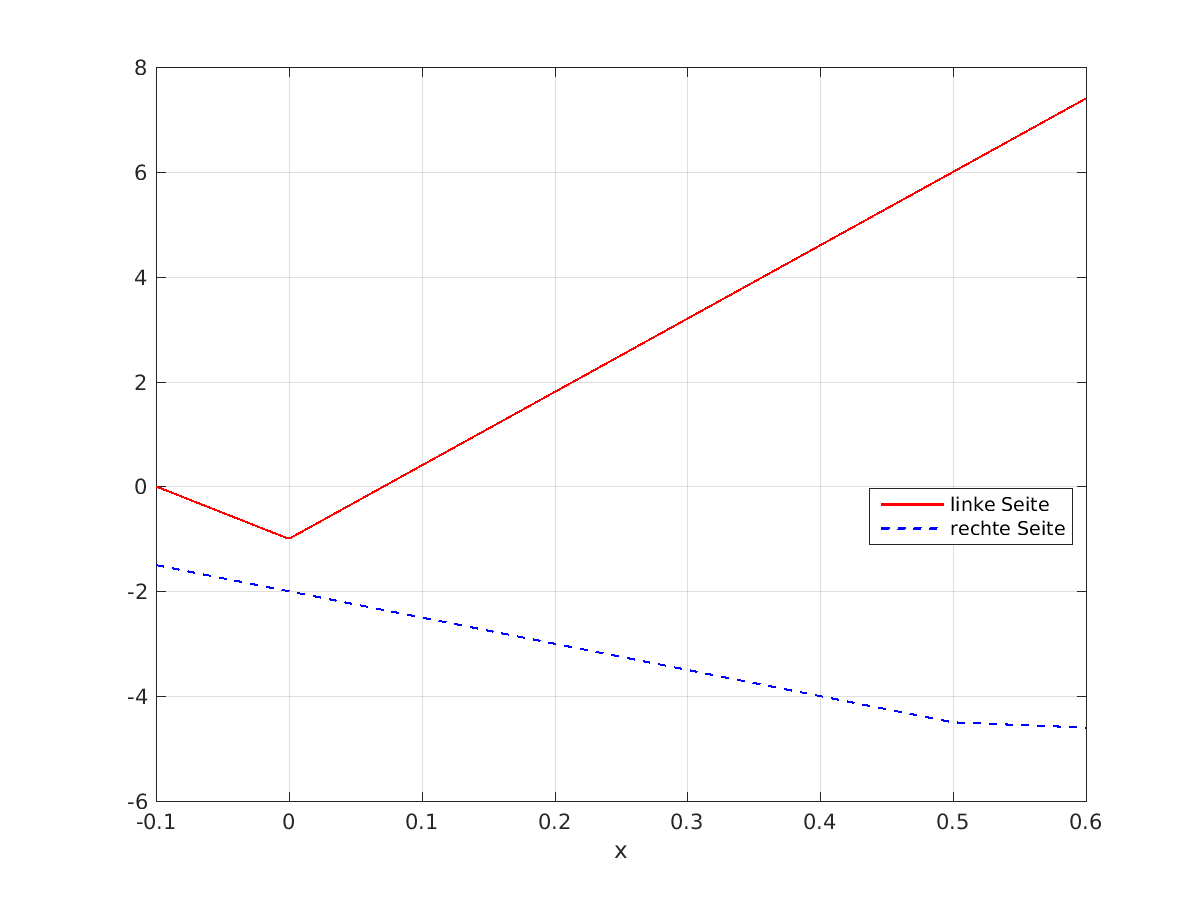
\includegraphics[width=0.8\linewidth]{Abb_zur_Ag_autogenerated_ineq_6.png} \end{center}
 
\else\relax\fi
 \end{MAufgabe}